% Options for packages loaded elsewhere
\PassOptionsToPackage{unicode}{hyperref}
\PassOptionsToPackage{hyphens}{url}
\PassOptionsToPackage{space}{xeCJK}
%
\documentclass[
]{report}
\usepackage{amsmath,amssymb}
\usepackage{lmodern}
\usepackage{iftex}
\ifPDFTeX
  \usepackage[T1]{fontenc}
  \usepackage[utf8]{inputenc}
  \usepackage{textcomp} % provide euro and other symbols
\else % if luatex or xetex
  \usepackage{unicode-math}
  \defaultfontfeatures{Scale=MatchLowercase}
  \defaultfontfeatures[\rmfamily]{Ligatures=TeX,Scale=1}
  \ifXeTeX
    \usepackage{xeCJK}
    \setCJKmainfont[]{Microsoft YaHei}
  \fi
  \ifLuaTeX
    \usepackage[]{luatexja-fontspec}
    \setmainjfont[]{Microsoft YaHei}
  \fi
\fi
% Use upquote if available, for straight quotes in verbatim environments
\IfFileExists{upquote.sty}{\usepackage{upquote}}{}
\IfFileExists{microtype.sty}{% use microtype if available
  \usepackage[]{microtype}
  \UseMicrotypeSet[protrusion]{basicmath} % disable protrusion for tt fonts
}{}
\makeatletter
\@ifundefined{KOMAClassName}{% if non-KOMA class
  \IfFileExists{parskip.sty}{%
    \usepackage{parskip}
  }{% else
    \setlength{\parindent}{0pt}
    \setlength{\parskip}{6pt plus 2pt minus 1pt}}
}{% if KOMA class
  \KOMAoptions{parskip=half}}
\makeatother
\usepackage{xcolor}
\usepackage[margin=1in]{geometry}
\usepackage{longtable,booktabs,array}
\usepackage{calc} % for calculating minipage widths
% Correct order of tables after \paragraph or \subparagraph
\usepackage{etoolbox}
\makeatletter
\patchcmd\longtable{\par}{\if@noskipsec\mbox{}\fi\par}{}{}
\makeatother
% Allow footnotes in longtable head/foot
\IfFileExists{footnotehyper.sty}{\usepackage{footnotehyper}}{\usepackage{footnote}}
\makesavenoteenv{longtable}
\usepackage{graphicx}
\makeatletter
\def\maxwidth{\ifdim\Gin@nat@width>\linewidth\linewidth\else\Gin@nat@width\fi}
\def\maxheight{\ifdim\Gin@nat@height>\textheight\textheight\else\Gin@nat@height\fi}
\makeatother
% Scale images if necessary, so that they will not overflow the page
% margins by default, and it is still possible to overwrite the defaults
% using explicit options in \includegraphics[width, height, ...]{}
\setkeys{Gin}{width=\maxwidth,height=\maxheight,keepaspectratio}
% Set default figure placement to htbp
\makeatletter
\def\fps@figure{htbp}
\makeatother
\setlength{\emergencystretch}{3em} % prevent overfull lines
\providecommand{\tightlist}{%
  \setlength{\itemsep}{0pt}\setlength{\parskip}{0pt}}
\setcounter{secnumdepth}{-\maxdimen} % remove section numbering
\usepackage{tikz}
\usepackage{circuitikz}
\usepackage{pgfplots}
\pgfplotsset{compat=1.18}
\usepackage{amssymb}
\DeclareMathOperator{\sgn}{sgn}
\DeclareMathOperator{\atan}{atan}
\DeclareMathOperator{\cand}{\mathbin{\!/\mkern-5mu/\!}}
\ifLuaTeX
  \usepackage{selnolig}  % disable illegal ligatures
\fi
\IfFileExists{bookmark.sty}{\usepackage{bookmark}}{\usepackage{hyperref}}
\IfFileExists{xurl.sty}{\usepackage{xurl}}{} % add URL line breaks if available
\urlstyle{same} % disable monospaced font for URLs
\hypersetup{
  pdftitle={電子學筆記},
  pdfauthor={林亦恩},
  hidelinks,
  pdfcreator={LaTeX via pandoc}}

\title{電子學筆記}
\author{林亦恩}
\date{}

\begin{document}
\maketitle

\hypertarget{ch1---ux96fbux5b50ux5143ux4ef6ux53caux6ce2ux5f62ux57faux672cux8a8dux8b58}{%
\chapter{CH1 -
電子元件及波形基本認識}\label{ch1---ux96fbux5b50ux5143ux4ef6ux53caux6ce2ux5f62ux57faux672cux8a8dux8b58}}

電子學: 討論荷電質點在氣體、真空或半導體中遷移的科學和工程學

\hypertarget{ux767cux5c55ux6b77ux53f2}{%
\section{發展歷史}\label{ux767cux5c55ux6b77ux53f2}}

\begin{enumerate}
\def\labelenumi{\arabic{enumi}.}
\tightlist
\item
  真空管時期(第一代)
\item
  電晶體時期(第二代)
\item
  積體電路時期(第三代) (SSI、MSI、LSI、VLSI)
\item
  微電腦時期(第四代) (ULSI)
\end{enumerate}

\hypertarget{ux7a4dux9ad4ux96fbux8defux5206ux985eux4f9dux6578ux91cf}{%
\section{積體電路分類(依數量)}\label{ux7a4dux9ad4ux96fbux8defux5206ux985eux4f9dux6578ux91cf}}

\begin{longtable}[]{@{}lll@{}}
\toprule()
名稱 & 邏輯閘數 & 零件數 \\
\midrule()
\endhead
SSI & \(12\) 以下 & \(100\) 以下 \\
MSI & \(12\)-\(100\) & \(100\)-\(1000\) \\
LSI & \(100\)-\(1000\) & \(1000\)-\(10000\) \\
VLSI & \(10^3\) - \(10^4\) & \(10^5\)-\(10^5\) \\
ULSI & \(10^4\) 以上 & \(10^5\) 以上 \\
\bottomrule()
\end{longtable}

從小到大排序:

\[
SSI < MSI < LSI < VLSI < ULSI
\]

\begin{itemize}
\tightlist
\item
  一個邏輯閘約等於10個元件數
\end{itemize}

\hypertarget{ux96fbux5b50ux5143ux4ef6ux7684ux61c9ux7528}{%
\section{電子元件的應用}\label{ux96fbux5b50ux5143ux4ef6ux7684ux61c9ux7528}}

4C:

\begin{itemize}
\tightlist
\item
  電腦(Computer)
\item
  通訊(Communication)
\item
  消費性電子(Consumer Electronics)
\item
  汽車電子(Car Electronics)
\end{itemize}

\hypertarget{ux57faux672cux6ce2ux5f62ux8a8dux8b58}{%
\section{基本波形認識}\label{ux57faux672cux6ce2ux5f62ux8a8dux8b58}}

\[
v(t) = V_m
\]

\(V_m\)是波型的最大值,也是波型的最低值

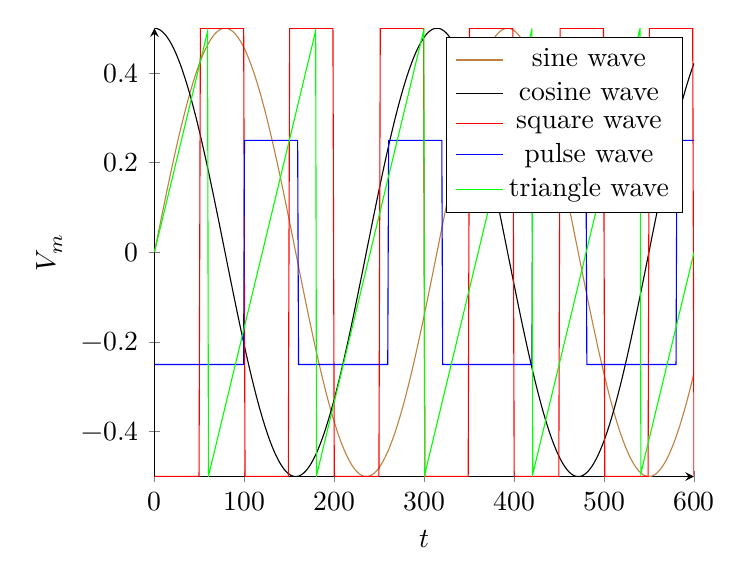
\begin{tikzpicture}
\begin{axis}[
    axis lines = left,
    xlabel = \(t\),
    ylabel = \( V_m\)
]
\addplot[color=brown, domain=0:600, samples=600] {sin(deg(x/50))/2};
\addlegendentry{sine wave}
\addplot[color=black, domain=0:600, samples=600] {cos(deg(x/50))/2};
\addlegendentry{cosine wave}
\addplot[color=red, domain=0:600, 
    samples=400] {(mod(x, 100) >= 50)-0.5};
\addlegendentry{square wave}
\addplot[color=blue, domain=0:600, samples=600] {((mod(x, 160) >= 100)/2)-0.25};
\addlegendentry{pulse wave}
\addplot[color=green, domain=0:600, samples=600] {5*x - floor(5*x + 0.5)};
\addlegendentry{triangle wave}
\end{axis}
\end{tikzpicture}

\hypertarget{ux76f4ux6d41dc-direct-current}{%
\subsection{直流(DC, Direct
Current)}\label{ux76f4ux6d41dc-direct-current}}

\begin{tikzpicture}
\begin{axis}
\addplot[domain=0:100, samples=100, color=blue]{1};
\end{axis}
\end{tikzpicture}

直流的正負極性不隨時間改變

\begin{itemize}
\tightlist
\item
  穩定直流: 大小(震幅)不變
\item
  脈動直流: 大小(震幅)隨時間改變
\end{itemize}

\hypertarget{ux4ea4ux6d41}{%
\subsection{交流}\label{ux4ea4ux6d41}}

交流的正負極性和震幅隨時間改變

常見交流波: 弦波、脈波、三角波、方波等

\hypertarget{ux5f26ux6ce2sine-wave}{%
\subsubsection{弦波(sine wave)}\label{ux5f26ux6ce2sine-wave}}

傅立葉分析: \textbf{弦波是基本訊號波形}

\[
v(t) = \sin(2 \pi f t)
\]

f: 頻率 t: 秒

角頻率

\[
\omega = 2 \pi f
\]

瞬時表示式

\[
v(t) = V_m \sin (\omega t + \theta)
\]

sin和cos的轉換

\[
V_m sin(\theta + 90) = V_m \cos \theta
\]

\hypertarget{ux8108ux6ce2pulse-wave}{%
\subsubsection{脈波(pulse wave)}\label{ux8108ux6ce2pulse-wave}}

脈波傅里葉級數展開為

\[
x(t)=A{\frac {\tau }{T}}+{\frac {2A}{\pi }}\sum _{n=1}^{\infty }\left({\frac {1}{n}}\sin \left(\pi n{\frac {\tau }{T}}\right)\cos \left(2\pi nft\right)\right)
\]

只有高準位(High)和低準位(Low)變化的波,通常用來測試放大器的頻率響應

工作週期

\[
V_{av} = \frac{t_H}{T} \times 100\%
\]

\begin{itemize}
\tightlist
\item
  方波: 工作週期為50\%
\item
  窄脈波: 工作週期小於50\%
\item
  寬脈波:工作週期大於50\%
\end{itemize}

\hypertarget{ux65b9ux6ce2square-wave}{%
\subsubsection{方波(square wave)}\label{ux65b9ux6ce2square-wave}}

方波可以視為取正弦波的正負號: 如果正弦波在那個時間大於零,則方波位於高()

用sgn(sign)函數表示

\[
x(t)=\sgn(\sin 2\pi ft)
\]

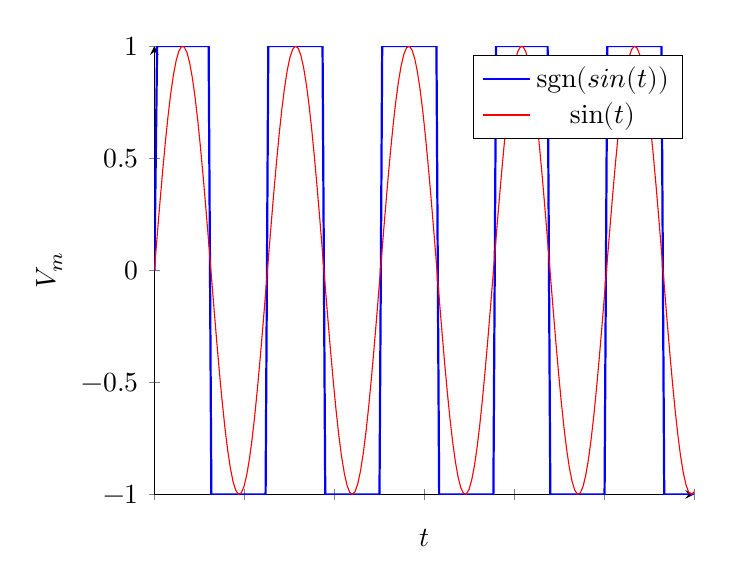
\begin{tikzpicture}
\begin{axis}[
    axis lines = left,
    xlabel = \(t\),
    ylabel = \( V_m\),
    xticklabels={},
    domain=0:30
]
\addplot[color=blue, samples=200, thick]{sign(sin(deg(x)))};
\addlegendentry{$\sgn(sin(t))$}
\addplot[color=red, samples=200]{sin(deg(x))};
\addlegendentry{$\sin(t)$}
\end{axis}
\end{tikzpicture}

或用floor函數表示

\[
x(t)=2\left(2\lfloor ft\rfloor -\lfloor 2ft\rfloor \right)+1
\]

\hypertarget{ux4e09ux89d2ux6ce2triangle-wave}{%
\subsubsection{三角波(triangle
wave)}\label{ux4e09ux89d2ux6ce2triangle-wave}}

範圍在 {[}0,1{]} 的三角波

\[
x(t)=2\left|{\frac {t}{p}}-\left\lfloor {\frac {t}{p}}+{\frac {1}{2}}\right\rfloor \right|
\]

a: 振幅 p: 週期

範圍在 {[}−1,1{]} 的三角波

\[
x(t)=2\left|2\left({\frac {t}{p}}-\left\lfloor {\frac{t}{p}}+{\frac{1}{2}}\right\rfloor \right)\right|-1.
\]

用取模運算表示

\[
y(x)={\frac {4a}{p}}\left|\left(\left(x-{\frac {p}{4}}\right){b \mod {p}}\right)-{\frac {p}{2}}\right|-a.
\]

用正弦波表示

\[
x(t)=\int _{0}^{t}sgn \left(\sin {\frac{u}{p}}\right)\,du.
\]

用三角函數表示

\[
y(x)={\frac {2a}{\pi }}\arcsin \left(\sin \left({\frac {2\pi }{p}}x\right)\right).
\]

用線性函數表示

\[
x(t)={\frac {4}{p}}\left(t-{\frac {p}{2}}\left\lfloor {\frac {2t}{p}}+{\frac {1}{2}}\right\rfloor \right)(-1)^{\left\lfloor {\frac {2t}{p}}+{\frac {1}{2}}\right\rfloor }
\]

三角波傅里葉級數展開為

\[
\begin{aligned}
x_{\mathrm {triangle} }(t)&{}={\frac {8}{\pi ^{2}}}\sum _{i=0}^{N-1}(-1)^{i}n^{-2}\sin \left(2\pi f_{0}nt\right)
\end{aligned}
\]

N: 要包含在近似值中的諧波數 t: 時間 \(f_0\): 基頻 i: 諧波標籤

應用於掃描控制電路,以上升時依上升斜率增加,下降時依下降斜率減少

上下斜率相等為正三角波,下降斜率為無限大(垂直)為掃描鋸齒波

\hypertarget{ux92f8ux9f52ux6ce2sawtooth-wave}{%
\subsection{鋸齒波(sawtooth
wave)}\label{ux92f8ux9f52ux6ce2sawtooth-wave}}

鋸齒波傅里葉級數展開為

\[
x_{\mathrm {sawtooth} }(t)={\frac {2}{\pi }}\sum _{k=1}^{\infty }{(-1)}^{k}{\frac {\sin(2\pi kft)}{k}}
\]

用取模運算表示

\[
v(t) = 2 (ft \% \frac{1}{f})f - 1
\]

鋸齒波可以用 \(\tan^-1\) (\(\arctan\)、\(\atan\))
來取的正弦波的角度(\(\frac{y}{x}\)),隔一段時間又歸零,不斷循環

\[
\tan^{-1(tan(t))}
v(t) = \tan^-1 (tag(t))
\]

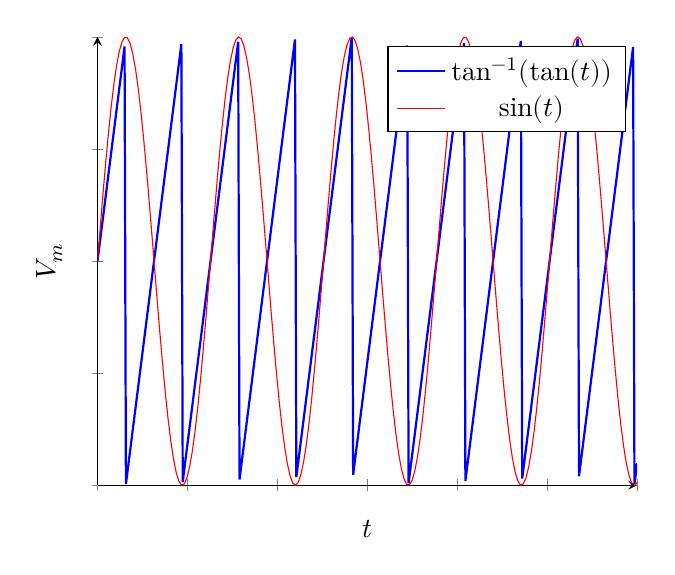
\begin{tikzpicture}
\begin{axis}[
    axis lines = left,
    xlabel = \(t\),
    ylabel = \( V_m\),
    xticklabels={},
    yticklabels={},
    domain=0:30
]
\addplot[color=blue, samples=400, thick]{atan(tan(deg(x)))/90};
\addlegendentry{$\tan^{-1}(\tan(t))$}
\addplot[color=red, samples=200]{sin(deg(x))};
\addlegendentry{$\sin(t)$}
\end{axis}
\end{tikzpicture}

可以使用取模函數,讓波型重複兩次才改變正負

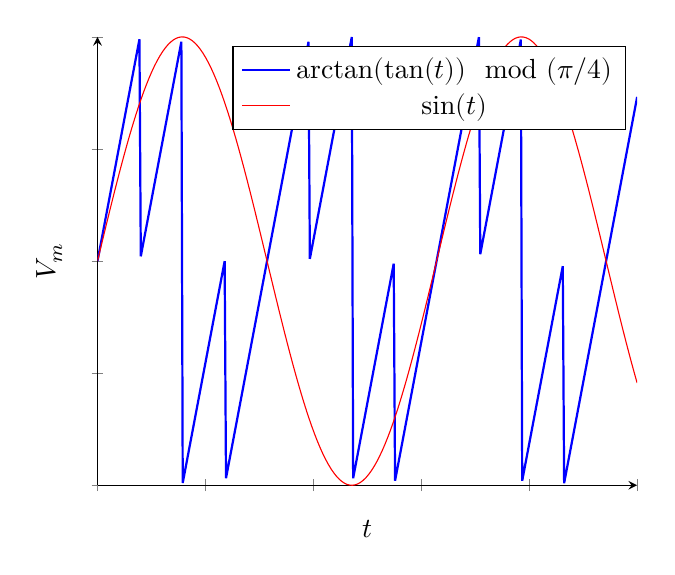
\begin{tikzpicture}
\begin{axis}[
    axis lines = left,
    xlabel = \(t\),
    ylabel = \( V_m\),
    xticklabels={},
    yticklabels={},
    domain=0:10
]
\addplot[color=blue, samples=400, thick]{mod(atan(tan(deg(x))), 45)/45};
\addlegendentry{$\arctan(\tan(t)) \mod (\pi / 4)$}
\addplot[color=red, samples=200]{sin(deg(x))};
\addlegendentry{$\sin(t)$}
\end{axis}
\end{tikzpicture}

\hypertarget{ux5e73ux5747ux503cux548cux6709ux6548ux503c}{%
\subsection{平均值和有效值}\label{ux5e73ux5747ux503cux548cux6709ux6548ux503c}}

平均值、平均數(Mean, Average)(\(V_{av}\)):
波形在週期內每個時間的瞬間值的總和和週期的比值

\[
{\overline {x}}={\frac {1}{n}}\left(\sum _{i=1}^{n}{x_{i}}\right)={\frac {x_{1}+x_{2}+\cdots +x_{n}}{n}}
\]

\[
V_{av} = \frac{V_1 \Delta t_1 + V_2 \Delta t_2 + \cdots}{T}
\]

\begin{itemize}
\tightlist
\item
  有效值(\(V_{rms}\), \(V_{eff}\))、均方根值(root square sum):
  讓一個交流電流電壓和一個直流電壓分別加到相同的電阻上,如果在相同周期內產生的熱量相等,那直流電壓的值就是交流電壓的有效值
\end{itemize}

電壓和電阻產生的功率公式

\[
P = \frac{V^2}{R}
\]

在交流電裡,有效值為

\[
V_{rms} = \sqrt{\frac{1}{2\pi}\int_{0}^{2\pi} v(t)^2  \mathrm{d}t}
\]

或者

\[
V_{rms} = \frac{{V_1}^2 \Delta t_1 + {V_2}^2 \Delta t_2 + \cdots}{T}
\]

波峰因數(crest factor, CF)

\[
CF = \frac{V_m}{V_{rms}}
\]

波形因素(form factor, FF)

\[
FF = \frac{V_rms}{V_{av}}
\]

當已知 \(V_m\) 時,各個波形的表格

\begin{longtable}[]{@{}
  >{\raggedright\arraybackslash}p{(\columnwidth - 8\tabcolsep) * \real{0.2143}}
  >{\raggedright\arraybackslash}p{(\columnwidth - 8\tabcolsep) * \real{0.2143}}
  >{\raggedright\arraybackslash}p{(\columnwidth - 8\tabcolsep) * \real{0.2143}}
  >{\raggedright\arraybackslash}p{(\columnwidth - 8\tabcolsep) * \real{0.2143}}
  >{\raggedright\arraybackslash}p{(\columnwidth - 8\tabcolsep) * \real{0.1429}}@{}}
\toprule()
\begin{minipage}[b]{\linewidth}\raggedright
波形
\end{minipage} & \begin{minipage}[b]{\linewidth}\raggedright
平均值
\end{minipage} & \begin{minipage}[b]{\linewidth}\raggedright
有效值
\end{minipage} & \begin{minipage}[b]{\linewidth}\raggedright
波峰因數CF
\end{minipage} & \begin{minipage}[b]{\linewidth}\raggedright
FF波形因素
\end{minipage} \\
\midrule()
\endhead
穩定直流 & \(V_m\) & \(V_m\) & \(1\) & \(1\) \\
方波 & \(V_m\) & \(V_m\) & \(1\) & \(1\) \\
三角波 & \(\frac{V_m}{2}\) & \(\frac{V_m}{\sqrt{3}}\) & \(\sqrt{3}\) &
\(\frac{2}{\sqrt{3}}\) \\
弦波 & \(\frac{2}{\pi}V_m\) & \(\frac{V_m}{\sqrt{2}}\) & \(\sqrt{2}\) &
\(\frac{\pi}{2 \sqrt{2}}\) \\
\bottomrule()
\end{longtable}

\begin{itemize}
\tightlist
\item
  弦波、方波、三角波全波的平均值為0,以正半週計算
\end{itemize}

\hypertarget{ux4ea4ux76f4ux6d41ux6df7ux548cux5f26ux6ce2}{%
\subsection{交直流混和弦波}\label{ux4ea4ux76f4ux6d41ux6df7ux548cux5f26ux6ce2}}

\begin{tikzpicture}
\begin{axis}[
    ymin = 0,
    ymax = 4,
    axis lines = left,
    xlabel = \(t\),
    ylabel = {\(v(t) = 2 + sin(deg(t))\)}]
\addplot[color=red, thick, domain=0:10, samples=100] plot {2 + sin(deg(\x))};
\end{axis}
\end{tikzpicture}

一個複雜的交直流混和弦波的順時表示式為

\[
v(t) = V_{dc} + a\sin({\omega}_1 t + {\theta}_1) + b\sin({\omega}_2 t + {\theta}_2 + \cdots)
\]

則全週期的平均值為 \(V_(dc)\),有效值為

\[
V_rms = \sqrt{V_dc ^ 2 + {\frac{a}{\sqrt{2}}}^2} + {\frac{b}{\sqrt{2}}}^2 + \cdots
\]

\hypertarget{ux55aeux4f4dux500dux6578ux7b26ux865fux7684ux610fux7fa9}{%
\section{單位倍數符號的意義}\label{ux55aeux4f4dux500dux6578ux7b26ux865fux7684ux610fux7fa9}}

\begin{longtable}[]{@{}lll@{}}
\toprule()
符號 & 符號 & 10的倍數 \\
\midrule()
\endhead
yocto & y & −24 \\
zepto & z & −21 \\
atto & a & −18 \\
femto & f & −15 \\
pico & p & −12 \\
nano & n & −9 \\
micro & \(μ\) & −6 \\
milli & m & −3 \\
centi & c & −2 \\
deci & d & −1 \\
deca & da & 1 \\
hecto & h & 2 \\
kilo & k & 3 \\
mega & M & 6 \\
giga & G & 9 \\
tera & T & 12 \\
peta & P & 15 \\
exa & E & 18 \\
zetta & Z & 21 \\
yotta & Y & 24 \\
\bottomrule()
\end{longtable}

\hypertarget{ch2---ux4e8cux6975ux9ad4ux8207ux61c9ux7528ux96fbux8def}{%
\chapter{CH2 -
二極體與應用電路}\label{ch2---ux4e8cux6975ux9ad4ux8207ux61c9ux7528ux96fbux8def}}

\hypertarget{ux539fux5b50ux6a21ux578b}{%
\section{原子模型}\label{ux539fux5b50ux6a21ux578b}}

\begin{itemize}
\tightlist
\item
  波爾原子模型 原子由電子(負電)、質子(正電)、中子(不代電)組成
  電子和質子構成原子核、外面是電子環繞。內層軌道的電子稱為\textbf{束縛電子}(bound
  electron),最外層為\textbf{價電子}(valence electron)
\item
  自由電子(free electron): 未被原子核及共價鏈所束縛的電子
\item
  傳導帶(conduction band):
  接近原子表面,所有在導帶中的電子均可經由外在的電場加速而形成電流
\item
  禁止帶(forbidden band): 傳導帶和價電帶之間
\item
  價電帶(valence band): 絕對零度下的固體中之電子所在最高能量的區域
\item
  化學晶體的八偶體學說: 價電帶有八個電子時,穩定性最高
\item
  價電子數小於4: 導體。例如: 銅、銀(導電性最佳)、金、石磨等
\item
  價電子數等於4: 半導體。例如: 矽(Si)、鍺(Ge)、砷化鎵(GaAs)
\item
  價電子數大於4: 絕緣體。例如: 石英、雲母、玻璃、空氣
\item
  電洞: 價電子獲得自由電子後離開而留下的空隙
\item
  能隙(energy gap): 電子由價電帶傳到傳導帶所需最小能量
\end{itemize}

電子組態: 每層所能容納最大電子數約為 \(2n^2\) ,n是軌道層次數

主層: 第一層: K(2) 第二層: L(8) 第三層: M(18) 第四層: N(32) 第五層:
O(50) 第六層: P(72) 第七層: Q(98)

副層: 第一層: s(2) 第二層: p(6) 第三層: d(10) 第四層: f(14)

\hypertarget{ux672cux8ceaux4e8cux6975ux9ad4}{%
\section{本質二極體}\label{ux672cux8ceaux4e8cux6975ux9ad4}}

定義: 四價二極體,沒有雜質

特性:

\begin{itemize}
\tightlist
\item
  負電阻溫度系數
\item
  電中性
\item
  絕對零度時如同絕緣體
\item
  室溫(25度)導通
\end{itemize}

\begin{longtable}[]{@{}ll@{}}
\toprule()
材料 & 能隙 \\
\midrule()
\endhead
Si & 1.11V \\
Ge & 0.66V \\
GaAs & 1.42V \\
\bottomrule()
\end{longtable}

\begin{itemize}
\tightlist
\item
  載子濃度
\end{itemize}

\[
{n_I}^2 = n \times p
\]

n為電子濃度,p為電洞濃度

\hypertarget{ux5916ux8ceaux534aux5c0eux9ad4}{%
\section{外質半導體}\label{ux5916ux8ceaux534aux5c0eux9ad4}}

原因:
因本質二極體電子-電動對濃度太低,而摻雜(doping)雜質元素的二極體,呈電中性

\begin{itemize}
\tightlist
\item
  P型:
  摻雜3價元素(硼B、鋁AI、鎵Ga、銦In),電洞數\textgreater 電子數,帶正電,為受體(acceptor)
\item
  N型: 摻雜5價元素(磷P, 砷As,
  銻Sb),電子數\textgreater 電洞數,帶負電,為施體(donnor)
\end{itemize}

\hypertarget{pnux4e8cux6975ux9ad4}{%
\section{PN二極體}\label{pnux4e8cux6975ux9ad4}}

\begin{itemize}
\tightlist
\item
  二極體電路符號
\end{itemize}

\begin{circuitikz}
\draw (0,0)
  to [diode] (0, 3);
\draw (2,0)
  to [full diode] (2, 3);
\end{circuitikz}

將P和N型變導體串在一起

特性:

\begin{itemize}
\tightlist
\item
  P為正,N為負
\item
  \(I_F\) 擴散電流: 由P往N流
\item
  \(I_S\) 飄移電流(逆向飽和電流): 由N往P流
\item
  未加偏壓: \(I_D = I_F - I_S = 0\),無電流
\item
  順向偏壓: (條件: 輸入電壓 \(V_D\) 大於切入電壓\(V_{DR}\) 時)
  \(I_D = I_F - I_S = I_S e^{\frac{V_D}{\eta V_T}}\),空乏區變小
\item
  逆向偏壓: \(I_F = 0\),空乏區變大,\(I_D = -I_S\)
\item
  崩潰: 逆向偏壓大於崩潰電壓(breakdown
  voltage),破壞二極體的共價結構,產生大量電流,二極體可能燒毀
\item
  切入電壓: \(V_{Br}\)

  \begin{itemize}
  \tightlist
  \item
    Si: 0.6V - 0.7V
  \item
    Ge: 0.2V - 0.3V
  \item
    GaAs: 1.1V - 1.2V
  \end{itemize}
\item
  靜態電阻:
\end{itemize}

\[
R_{DC} = \frac{V_{DQ}}{I_{DQ}}
\]

\begin{itemize}
\tightlist
\item
  動態電阻
\end{itemize}

\[
r_d = \frac{\eta V_T}{I_{DQ}} \approx \frac{V_T}{I_{DQ}}
\]

在室溫300K下,\(V_T \approx 26mV\)

\[
r_d = \frac{26mV}{I_{DQ}}
\]

室溫25度下,\(V_T \approx 25mV\)

\begin{itemize}
\tightlist
\item
  本體電阻(bulk resistance)(或稱分布電阻)
\end{itemize}

\[
r_B = \frac{V_{DQ} - V_{DR}}{I_{DQ}}
\]

\begin{itemize}
\tightlist
\item
  空乏電容(transition-region capacitance)
\end{itemize}

\[
C_T = \epsilon \frac{A}{W}
\]

\(\epsilon\)為介電常數( \(\frac{F}{m}\) ),A為截面積( \(m^2\)
),W為空乏區寬度(\(m\))

\begin{itemize}
\tightlist
\item
  擴散電容
\end{itemize}

\[
C_D = \frac{\tau \times I_{DQ}}{\eta V_{T}} =
\frac{\tau}{r_d}
\]

\begin{itemize}
\item
  溫度特性:
  每上升1度,切入電壓約下降1mV到2.5mV,逆向飽和電流隨每溫度上生10度增加一倍(\(2^{\frac{\Delta T}{10}}\))
\item
  等效電路
\end{itemize}

\begin{enumerate}
\def\labelenumi{\arabic{enumi}.}
\tightlist
\item
  理想: 開關
\end{enumerate}

\begin{circuitikz}
\draw (0,0)
  to [full diode] (0, 5);
\draw (5, 0)
  to [cute open switch] (5, 5);
\end{circuitikz}

\begin{enumerate}
\def\labelenumi{\arabic{enumi}.}
\setcounter{enumi}{1}
\tightlist
\item
  簡化: 開關 + 切入電壓
\end{enumerate}

\begin{circuitikz}
\draw (0,0)
  to [full diode] (0, 5);
\draw (5, 0)
  to [battery2, v<=$v_{DR}$] (5, 2.5)
  to [cute open switch] (5, 5);
\end{circuitikz}

\begin{enumerate}
\def\labelenumi{\arabic{enumi}.}
\setcounter{enumi}{2}
\tightlist
\item
  進階: 開關 + 切入電壓 + 電阻
\end{enumerate}

\begin{circuitikz}
\draw (0,0)
  to [full diode] (0, 6);
\draw (5, 0)
  to [battery2, v<=$v_{DR}$] (5, 2)
  to [R=$r_B$] (5, 4)
  to [cute open switch] (5, 6);
\end{circuitikz}

\hypertarget{ux6574ux6d41ux96fbux8def}{%
\section{整流電路}\label{ux6574ux6d41ux96fbux8def}}

\begin{itemize}
\tightlist
\item
  圖: 半波整流
\end{itemize}

\begin{circuitikz}
\draw (0, 0)
  to [sI=$V_S$] (0, 3)
  to [full diode, l_=$D_1$, -*](3, 3)
  to [R=$R_L$, -*] (3, 0);
\draw (3, 3)
  to [short, -o] (4, 3)
  to [open, v=$V_o$, -o] (4, 0)
  to [short] (0, 0);
\end{circuitikz}

\begin{itemize}
\tightlist
\item
  圖: 全波整流
\end{itemize}

\begin{circuitikz}
\draw (0, 0)
  to [sI<=$V_S1$] (0, 3)
  to [diode, l_=$D_1$, -*] (3, 3)
  to [short, i<=$i_1$,-*] (3, 0)
  to [R=$R_L$, v=$V_o$] (0, 0);
\draw (0, -3)
  to [full diode, l_=$D_2$] (3, -3)
  to [short, i=$i_2$, -*] (3, 0);
\draw (0, -3)
  to [sI<=$V_S2$] (0, 0);
\end{circuitikz}

\begin{itemize}
\tightlist
\item
  圖: 橋式整流
\end{itemize}

\begin{circuitikz}
\draw (0, 0)
  to [R=$R_L$, v=$V_o$] (6, 0)
  to [full diode, l_=$D_2$] (3, 3)
  to [diode, l_=$D_1$] (0, 0);
\draw (6, 0)
  to [diode, l_=$D_4$] (3, -3)
  to [full diode, l_=$D_3$] (0, 0);
\draw (3, 3)
  to [short] (-2.7, 3);
\draw (3, -3)
  to [short] (-2.7, -3);
\draw (-1.7, 3)
  to [open, v=$V_S$] (-1.7, -3);
\draw (-2.7, 3)
 to node[transformer core] {} (-2.7, -3);
\end{circuitikz}

\begin{longtable}[]{@{}
  >{\raggedright\arraybackslash}p{(\columnwidth - 6\tabcolsep) * \real{0.2500}}
  >{\raggedright\arraybackslash}p{(\columnwidth - 6\tabcolsep) * \real{0.2500}}
  >{\raggedright\arraybackslash}p{(\columnwidth - 6\tabcolsep) * \real{0.2500}}
  >{\raggedright\arraybackslash}p{(\columnwidth - 6\tabcolsep) * \real{0.2500}}@{}}
\toprule()
\begin{minipage}[b]{\linewidth}\raggedright
特性
\end{minipage} & \begin{minipage}[b]{\linewidth}\raggedright
半波整流
\end{minipage} & \begin{minipage}[b]{\linewidth}\raggedright
全波整流
\end{minipage} & \begin{minipage}[b]{\linewidth}\raggedright
橋式整流
\end{minipage} \\
\midrule()
\endhead
輸出\(V_o(p)\) & \(V_S(m)\) & \(V_S(m)\) & \(V_S(m)\) \\
\(V_{o(dc)}\) & \(\frac{V_{o(p)}}{\pi}\) & \(\frac{2V_{o(p)}}{\pi}\) &
\(\frac{2V_{o(p)}}{\pi}\) \\
\(V_{o(rms)}\) & \(\frac{|V_{o(p)}|}{2}\) &
\(\frac{|V_{o(p)}|}{\sqrt{2}}\) & \(\frac{|V_{o(p)}|}{\sqrt{2}}\) \\
頻率f & \(f_s\) & \(2f_s\) & \(2f_s\) \\
週期T & \(T_S\) & \(\frac{T_S}{2}\) & \(\frac{T_S}{2}\) \\
二極體PIV & \(V_S(M)\) & \(2V_S(M)\) & \(2V_S(M)\) \\
純整流電路蓮波因數r\% & 121\% & 48\% & 48\% \\
\bottomrule()
\end{longtable}

\hypertarget{ux6ffeux6ce2ux96fbux8def}{%
\section{濾波電路}\label{ux6ffeux6ce2ux96fbux8def}}

\begin{itemize}
\tightlist
\item
  圖: 橋式整流電容濾波電路
\end{itemize}

\begin{circuitikz}
\ctikzset{inductors/width=1, inductors/scale=1.2}
\draw (0, 0)
  to [R=$R_L$, v=$V_o$] (6, 0)
  to [full diode, l_=$D_2$] (3, 3)
  to [diode, l_=$D_1$] (0, 0);
\draw (6, 0)
  to [diode, l_=$D_4$] (3, -3)
  to [full diode, l_=$D_3$] (0, 0);
\draw (3, 3)
  to [short] (-2.7, 3);
\draw (3, -3)
  to [short] (-2.7, -3);
\draw (-1.7, 3)
  to [open, v=$V_S$] (-1.7, -3);
\draw (-2.7, 3)
 to node[transformer core] {} (-2.7, -3);
\draw (6, 0)
  to [short] (6.7, 0)
  to [capacitor=$C$] (6.7, -2)
  to [ground] (6.7, -3);
\draw (6, 0)
  to [short, -o, l_=$V_o$] (9, 0);
\draw (8, 0)
  to [R=$R_L$] (8, -3)
  to [ground] (8, -3);
\end{circuitikz}

\begin{itemize}
\tightlist
\item
  蓮波電壓
\end{itemize}

輸出 = DC輸出 + 蓮波電壓(變動)

\begin{itemize}
\tightlist
\item
  蓮波電壓有效值
\end{itemize}

\[
V_{r(rms)} = \sqrt{{V_o}^2 - {V_{o(dc)}}^2}
\]

\begin{itemize}
\tightlist
\item
  蓮波因數百分比
\end{itemize}

\[
r\% = \frac{V_{r(rms)}}{V_{o(dc)}} \times 100\%
\]

\begin{itemize}
\tightlist
\item
  電容濾波: 整流輸出端並聯電容,讓波型接近直流,降低蓮波電壓

  \begin{itemize}
  \tightlist
  \item
    半波整流二極體PIV: \(2V_{s(m)}\) (2倍)
  \item
    全波整流二極體PIV: \(2V_{s(m)}\) (相同)
  \item
    橋式整流二極體PIV: \(V_{s(m)}\) (相同)
  \item
    頻率: 皆為 \(2f_s\)
  \item
    週期: 皆為 \(\frac{T_s}{2}\)
  \item
    電容時間常數 =
    \(R \times C\),提高電容或電阻可延長電容放電時間,降低蓮波電壓,輸出直流加大
  \end{itemize}
\item
  蓮波電壓有效值
\end{itemize}

蓮波峰對峰值

\[
V_{r(p-p)} = \Delta V \approx V_{o(p)} \frac{\times T_0}{C} = \frac{V_{o(p)}}{R_L \times C \times f_0}
\]

若蓮波接進鋸齒波,則有效值

\[
V_{r(rms)} = \frac{V_{r(pp)}}{2 \sqrt{3}} = \frac{V_{o(p)} \times T_0}{2\sqrt{3} \times R_L \times C} = \frac{V_{o(p)}}{2\sqrt{3} \times C \times f_0}
\]

\begin{itemize}
\item
  全波和橋式整流的\(f_0 = 2 f_s\),分母要承二
\item
  直流輸出
\end{itemize}

\[
V_{o(dc)} = V_{o(p)} - \frac{V_{r(p-p)}}{2}
\]

\begin{itemize}
\tightlist
\item
  蓮波因數

  \begin{itemize}
  \tightlist
  \item
    半波整流: \(\frac{0.48}{R_L \times C}\%\)
  \item
    全波和橋式整流: \(\frac{0.24}{R_L \times C}\%\)
  \end{itemize}
\end{itemize}

\hypertarget{ux7a3dux7d0dux4e8cux6975ux9ad4}{%
\section{稽納二極體}\label{ux7a3dux7d0dux4e8cux6975ux9ad4}}

\begin{itemize}
\tightlist
\item
  稽納二極體電路符號
\end{itemize}

\begin{circuitikz}
\draw (0,0) to [full Zener diode] (2,0); 
\end{circuitikz}

工作於崩潰區的二極體,應用於\textbf{穩壓}、保護電路、參考電壓電路

\begin{itemize}
\item
  稽納崩潰:
  主要發生在逆向偏壓大於6V以下,崩潰邊壓隨溫度上升而減少(負電阻溫度係數)
\item
  壘增崩潰:
  主要發生在逆向偏壓大於6V以上,崩潰邊壓隨溫度上升而增加(正電阻溫度係數)
\item
  稽納電壓(Zener voltage): 在二極體崩潰區時沒燒毀的情況的固定電壓
\item
  特性曲線
\end{itemize}

\[
r_s = \frac{\Delta V_Z}{\Delta I_Z} \approx \frac{V_Z - V_{ZK}}{I_Z - I_{ZK}}
\]

\begin{itemize}
\tightlist
\item
  等效電路: 電壓(\(V_Z\))
\item
  函電阻等效電路: 電壓(\(V_Z\)) + 稽納電阻(\(r_Z\))
\item
  稽納電流:
\end{itemize}

\begin{circuitikz}
\draw (0,0)
  to [short, -*](4, 0)
  to [full Zener diode, -*, l_=$V_Z$, i<=$I_Z$] (4, 3)
  to [R] (0, 3)
  to [battery, v=$V_S$, i<=$I$] (0, 0);
\draw (4, 0)
  to [short, -o] (6, 0);
\draw (4, 3)
  to [short, -o] (6, 3);
\draw (6, 0)
  to [open, v<=$V_o$](6, 3);
\end{circuitikz}

圖: 基納二極體加上電壓

\[
I_Z = \frac{V_S - V_Z}{R}
\]

圖: 基納二極體電源穩壓調整電路

\begin{circuitikz}
\draw (0, 0)
  to [short] (6, 0)
  to [full diode, l_=$D_1$, -*] (6, 2);
\draw (6, 4)
  to [diode, l_=$D_2$] (6, 2);
\draw (4, 2)
  to [full diode, l_=$D_3$, *-*] (4, 4)
  to [short] (0, 4);
\draw (4, 2)
  to [diode, l_=$D_4$, *-*] (4, 0);
\draw (6, 2)
  to [short] (7.5, 2)
  to [capacitor, l_=$C$] (7.5, 0)
  to node[ground]{} (7.5, -1);
\draw (7.5, 2)
  to [R=$R_S$] (9.5, 2)
  to [full Zener diode, l_=$V_Z$] (9.5, 0)
  to node[ground]{} (9.5, -1);
\draw (9.5, 2)
  to [short] (10.5, 2)
  to [R=$R_L$] (10.5, 0)
  to node[ground] {} (10.5, -1);
\draw (10.5, 2)
  to [short] (11, 2)
  to [short, -o, l_=$V_o$](11.2, 2);
\draw (6, 0)
  to [short, -o] (6.5, 0);
\draw (4, 2)
  to [short] (3, 2)
  to node[ground]{} (3, 1);
\draw (4, 4)
  to [short] (6, 4);
\draw (0, 0)
  to node[transformer core] {} (0, 4);
\draw (0.7, 0)
  to [open, v<=$V_S$] (0.7, 4);
\draw (-0.2, 4.5) node[] {11 : 1};
\draw (-1, 0)
  to [open, v<=$V_i$] (-1, 4);
\node[draw] at (-2.5, 2) {110V/60Hz};
\end{circuitikz}

\hypertarget{ux767cux5149ux4e8cux6975ux9ad4}{%
\section{發光二極體}\label{ux767cux5149ux4e8cux6975ux9ad4}}

發光二極體(light-emitting diode,
LED)是利用波爾定理把電能轉換成光能的電子元件

\begin{itemize}
\tightlist
\item
  冷性發光
\item
  發射的光波長約在 400nm到800nm之間
\item
  壽命長(一萬小時以上)
\item
  環保
\item
  耐震
\item
  可平面封裝
\item
  體積小
\item
  發熱量低
\item
  P-N
  接面加順向偏壓,使電子-電洞對移動,並空乏區複合,使電子由傳導帶移轉至價電帶而喪失能接,以散色光釋放出能量
\item
  紅外線:
  如果用在光感測器的光原,須搭配受光元件,將光轉換成電來使用,其分光感度主要在800
  - 900nm之間
\item
  有機方光二極體OLED(organic LED): 薄、壽命短、可彎曲、效率高
\end{itemize}

\hypertarget{ch3---ux96d9ux6975ux6027ux63a5ux9762ux4e8cux6975ux9ad4}{%
\chapter{CH3 -
雙極性接面二極體}\label{ch3---ux96d9ux6975ux6027ux63a5ux9762ux4e8cux6975ux9ad4}}

\begin{itemize}
\tightlist
\item
  電路符號一
\end{itemize}

\begin{circuitikz}
\draw (0,0)
  to node[npn]{} (0, 3);
\node[draw] at (-1, 0) {NPN Transistor};
\draw (2,0)
  to node[pnp]{} (2, 3);
\node[draw] at (3, 0) {PNP Transistor};
\end{circuitikz}

\begin{itemize}
\tightlist
\item
  電路符號二(圓圈)
\end{itemize}

\begin{circuitikz}
\draw (0,0)
  to node[npn, tr circle]{} (0, 3);
\node[draw] at (-1, 0) {NPN Transistor};
\draw (2,0)
  to node[pnp, tr circle]{} (2, 3);
\node[draw] at (3, 0) {PNP Transistor};
\end{circuitikz}

\begin{itemize}
\tightlist
\item
  電路符號三(圓圈+內部二極體)
\end{itemize}

\begin{circuitikz}
\draw (0,0)
  to node[npn, tr circle, bodydiode]{} (0, 3);
\node[draw] at (-1, 0) {NPN Transistor};
\draw (2,0)
  to node[pnp, tr circle, bodydiode]{} (2, 3);
\node[draw] at (3, 0) {PNP Transistor};
\end{circuitikz}

\begin{longtable}[]{@{}lll@{}}
\toprule()
特性 & PNP & NPN \\
\midrule()
\endhead
多數載子 & 電洞 & 電子 \\
少數載子 & 電子 & 電洞 \\
濃度 & \(E > B > C\) & \\
寬度 & \(C > E > B\) (B極越薄,放大率越大 & \\
頻率響應 & NPN 優於 PNP(電子移動速度較快) & \\
\bottomrule()
\end{longtable}

\begin{itemize}
\tightlist
\item
  NPN內部構造圖
\end{itemize}

\includegraphics{NPN.png}

\begin{itemize}
\tightlist
\item
  增加電流放大率,讓E極濃度增加或B極寬度變窄
\item
  射極(Emitter, E),集極(Collector, C),基極(Base, B)
\item
  障壁電壓 \(V_{BEr} \approx 0.7V\),\(V_{BCr} \approx 0.5V\)
\item
  BJT是主動元件
\end{itemize}

\hypertarget{bjtux56dbux7a2eux5de5ux4f5cux6a21ux5f0f}{%
\section{BJT四種工作模式}\label{bjtux56dbux7a2eux5de5ux4f5cux6a21ux5f0f}}

\begin{longtable}[]{@{}llll@{}}
\toprule()
工作模式 & BE接面 & BC接面 & 應用電路 \\
\midrule()
\endhead
順向主動區(active) & 順向偏壓 & 逆向偏壓 & 放大電路 \\
逆向主動區(reverse active) & 逆向偏壓 & 順向偏壓 & 邏輯交換電路 \\
飽和區(saturation) & 順向偏壓 & 順向偏壓 & 開關為ON \\
截止區(cut-off) & 逆向偏壓 & 逆向偏壓 & 開關為OFF \\
\bottomrule()
\end{longtable}

\begin{itemize}
\tightlist
\item
  截止區條件:
\end{itemize}

\begin{equation*}
\begin{split}
& I_B = 0 \\
& I_C = I_{CEO} \\
& V_{BE} < V_{BEr} \\
& V_{CE} = V_{CC}
\end{split}
\end{equation*}

\begin{itemize}
\tightlist
\item
  飽和區條件:
\end{itemize}

\[
I_{C} = \beta I_B > I_{C(sat)}
\]

\(V_{CE}\) 約在 0.2V 以下

\begin{itemize}
\item
  工作區時 \(V_{CE} \approx 0.2V - V_{CC}\) , \(I_C = \beta I_B\)
\item
  常見的電晶體各點電壓值
\end{itemize}

\begin{longtable}[]{@{}
  >{\raggedright\arraybackslash}p{(\columnwidth - 10\tabcolsep) * \real{0.1667}}
  >{\raggedright\arraybackslash}p{(\columnwidth - 10\tabcolsep) * \real{0.1667}}
  >{\raggedright\arraybackslash}p{(\columnwidth - 10\tabcolsep) * \real{0.1667}}
  >{\raggedright\arraybackslash}p{(\columnwidth - 10\tabcolsep) * \real{0.1667}}
  >{\raggedright\arraybackslash}p{(\columnwidth - 10\tabcolsep) * \real{0.1667}}
  >{\raggedright\arraybackslash}p{(\columnwidth - 10\tabcolsep) * \real{0.1667}}@{}}
\toprule()
\begin{minipage}[b]{\linewidth}\raggedright
材料
\end{minipage} & \begin{minipage}[b]{\linewidth}\raggedright
\(V_{CE(sat)}\)
\end{minipage} & \begin{minipage}[b]{\linewidth}\raggedright
\(V_{BE(sat)}\)
\end{minipage} & \begin{minipage}[b]{\linewidth}\raggedright
\(V_{BE(active)}\)
\end{minipage} & \begin{minipage}[b]{\linewidth}\raggedright
\(V_{BE(cut-in)}\)
\end{minipage} & \begin{minipage}[b]{\linewidth}\raggedright
\(V_{BE(cut-off)}\)
\end{minipage} \\
\midrule()
\endhead
矽Si & 0.2V & 0.8V & 0.7V & 0.5V & 0V \\
鍺Ge & 0.1V & 0.3V & 0.2V & 0.1V & -0.1V \\
\bottomrule()
\end{longtable}

\begin{itemize}
\tightlist
\item
  圖: BJT工作區域和電流、電壓的關係(作者: AlexHe34,連結:
  \url{https://zh.m.wikipedia.org/wiki/File:Current-Voltage_relationship_of_BJT_zh.png})
\end{itemize}

\includegraphics{BJT_work.png}

\hypertarget{bjtux7684ux4e09ux7a2eux5de5ux4f5cux7d44ux614b}{%
\section{BJT的三種工作組態}\label{bjtux7684ux4e09ux7a2eux5de5ux4f5cux7d44ux614b}}

\begin{longtable}[]{@{}
  >{\raggedright\arraybackslash}p{(\columnwidth - 12\tabcolsep) * \real{0.1471}}
  >{\raggedright\arraybackslash}p{(\columnwidth - 12\tabcolsep) * \real{0.1471}}
  >{\raggedright\arraybackslash}p{(\columnwidth - 12\tabcolsep) * \real{0.1471}}
  >{\raggedright\arraybackslash}p{(\columnwidth - 12\tabcolsep) * \real{0.1471}}
  >{\raggedright\arraybackslash}p{(\columnwidth - 12\tabcolsep) * \real{0.1471}}
  >{\raggedright\arraybackslash}p{(\columnwidth - 12\tabcolsep) * \real{0.1471}}
  >{\raggedright\arraybackslash}p{(\columnwidth - 12\tabcolsep) * \real{0.1176}}@{}}
\toprule()
\begin{minipage}[b]{\linewidth}\raggedright
工作組態
\end{minipage} & \begin{minipage}[b]{\linewidth}\raggedright
簡寫
\end{minipage} & \begin{minipage}[b]{\linewidth}\raggedright
全名
\end{minipage} & \begin{minipage}[b]{\linewidth}\raggedright
輸入端
\end{minipage} & \begin{minipage}[b]{\linewidth}\raggedright
輸出端
\end{minipage} & \begin{minipage}[b]{\linewidth}\raggedright
共接端
\end{minipage} & \begin{minipage}[b]{\linewidth}\raggedright
電流增益 \(A_i\)
\end{minipage} \\
\midrule()
\endhead
共射極組態 & CE & common-emitter & B極 & C極 & E極 &
\({\beta}_{dc} = \frac{I_C}{I_B}\) \\
共集極組態 & CC & common-collector & E極 & E極 & C極 &
\({\gamma}_{dc} = \frac{I_E}{I_B}\) \\
共基極組態 & CB & common-base & E極 & C極 & B極 &
\({\alpha}_{dc} = \frac{I_C}{I_E}\) \\
\bottomrule()
\end{longtable}

\begin{itemize}
\tightlist
\item
  C極不可當作輸入端
\item
  B極不可當作輸出端
\end{itemize}

\hypertarget{bjtux7684ux984dux5b9aux6700ux5927ux503c}{%
\section{BJT的額定最大值}\label{bjtux7684ux984dux5b9aux6700ux5927ux503c}}

CE、CB、CC的額定最大值分別為

\begin{equation*}
\begin{split}
& P_{C(max)} = V_{CE(max)} \times I_{C(max)} \\
& P_{C(max)} = V_{CB(max)} \times I_{C(max)} \\
& P_{C(max)} = V_{CE(max)} \times I_{C(max)}
\end{split}
\end{equation*}

\hypertarget{bjtux653eux5927ux5668ux589eux76ca}{%
\section{BJT放大器增益}\label{bjtux653eux5927ux5668ux589eux76ca}}

\begin{itemize}
\tightlist
\item
  定義: 輸出和輸入的比值
\item
  如過沒有特別說明,放大器一般指電壓放大器
\end{itemize}

\begin{equation*}
\begin{split}
& A_v = \frac{v_o}{v_i} \\
& A_i = \frac{v_o}{i_i} \\
& A_p = \frac{p_o}{p_i} = | A_v \times A_i |
\end{split}
\end{equation*}

\hypertarget{bjtux9806ux5411ux4e3bux52d5ux5340ux53c3ux6578}{%
\section{BJT順向主動區參數}\label{bjtux9806ux5411ux4e3bux52d5ux5340ux53c3ux6578}}

\begin{itemize}
\tightlist
\item
  多數載子來自E極
\item
  主要當作放大器
\item
  NPN時主要載子為電子流
\item
  PNP時主要載子為電洞流
\end{itemize}

\[
I_E = I_B + I_C
\]

電流參數

\begin{equation*}
\begin{split}
& {\alpha}_F = \frac{I_C}{I_E} \\
& {\beta}_F = \frac{I_C}{I_B}_F  \\
& {\gamma}_F = \frac{I_E}{ I_B} = 1 + β_F 
\end{split}
\end{equation*}

\begin{itemize}
\tightlist
\item
  \({\alpha}_F\) 為順向阿法(forward alpha)
\item
  \({\beta}_F\) 為順向貝塔(forward beta)
\item
  \({\gamma}_F\) 為順向伽馬(forward gamma)
\item
  \({\beta}_F\) 大於1,約在50以上
\item
  \({\alpha}_F\) 小於1,約在0.98以上
\item
  \({\gamma}_F\) 比 \(β_F\)大1
\end{itemize}

\hypertarget{bjtux9006ux5411ux4e3bux52d5ux5340ux53c3ux6578}{%
\section{BJT逆向主動區參數}\label{bjtux9006ux5411ux4e3bux52d5ux5340ux53c3ux6578}}

\begin{itemize}
\tightlist
\item
  一般不會單獨使用,而是搭配順向主動區,如數位邏輯的TTL邏輯電路
\item
  多數載子來自C極
\end{itemize}

\[
I_C = I_B + I_E
\]

電流參數

\begin{equation*}
\begin{split}
& {\alpha}_R = \frac{I_E}{I_C} \\
& {\beta}_R = \frac{I_E}{I_B}_F 
\end{split}
\end{equation*}

\begin{itemize}
\tightlist
\item
  \({\alpha}_R\) 為逆向阿法(reverse alpha)
\item
  \({\beta}_R\) 為逆向貝塔(reverse beta)
\end{itemize}

\hypertarget{bjtux76f4ux6d41ux5206ux6790---ux627eux76f4ux6d41ux5de5ux4f5cux9ede}{%
\section{BJT直流分析 -
找直流工作點}\label{bjtux76f4ux6d41ux5206ux6790---ux627eux76f4ux6d41ux5de5ux4f5cux9ede}}

當BJT當作放大器時

\begin{itemize}
\tightlist
\item
  偏壓(bias): 施加在主動元件各極的直流電源
\item
  直流工作點、靜態工作點(quiescent operating
  point),俗稱Q點,位於作用區內
\item
  找出Q點的 \(V_{BEQ}\) 和 \(I_{CQ}\)
\end{itemize}

\hypertarget{bjt-ux653eux5927ux96fbux8def}{%
\section{BJT 放大電路}\label{bjt-ux653eux5927ux96fbux8def}}

分為

\begin{itemize}
\tightlist
\item
  共射極放大電路
\item
  共極極放大電路
\item
  共基極放大電路
\end{itemize}

\hypertarget{ux6eabux5ea6ux5c0dbjtux7684ux5f15ux97ff}{%
\section{溫度對BJT的引響}\label{ux6eabux5ea6ux5c0dbjtux7684ux5f15ux97ff}}

\begin{itemize}
\tightlist
\item
  參考溫度對PN二極體的引響
\item
  BJT的 \(\beta\) 值隨溫度上升而變大
\item
  BJT的B、E兩端切入電壓 \(V_{BEr}\) 隨溫度上升一度下降 \(1mV\) -
  \$\$2.5mV
\end{itemize}

\[
I_C = \beta I_B + (1 + \beta) I_{CO}
\]

\(I_{CO}\) 為C、B端的漏電流(飄移電流 \(I_S\)),隨溫度上升10度而增加一倍

\hypertarget{bjt-ux76f4ux6d41ux504fux58d3ux96fbux8def}{%
\section{BJT
直流偏壓電路}\label{bjt-ux76f4ux6d41ux504fux58d3ux96fbux8def}}

\hypertarget{ux56faux5b9aux5f0fux504fux58d3fixed-base-bias}{%
\subsection{固定式偏壓(fixed base
bias)}\label{ux56faux5b9aux5f0fux504fux58d3fixed-base-bias}}

E 極為短路、C極和B極加上電阻

\begin{circuitikz}
\node[draw] at (0, -1) {fixed base bias};
\node[ground] at (0, 0) {};
\ctikzset{transistors/thickness=4, transistors/fill=cyan!30, transistor circle/relative thickness=0.25,}
\draw (0, 0)
  to [short, i=$I_E$] (0, 1)
  to node[npn, tr circle](N){} (0, 3)
  to [R=$R_C$, i<=$I_C$] (0, 5)
  to [short] (0, 6.9)
  to [short, l_=$V_{CC}$, -o] (0, 7);
\draw (N.circle base)
  to [short] (-2, 2)
  to [R=$R_B$, i<=$I_B$] (-2, 6)
  to [short, -*] (0, 6);
\end{circuitikz}

\begin{circuitikz}
\draw (0, -1.5)
  to [short] (7, -1.5)
  to [battery2, v<=$V_{CC}$] (7, -9)
  to [short, -*] (4, -9);
\node[ground] at (4, -9) {};
\draw (0, -1.5)
  to [R=$R_B$] (0, -4)
  to [short, i=$I_B$](2, -4) 
  to [battery2, v<=$V_{BEr}$] (2, -6)
  to [short, -*] (4, -6)
  to [short, i=$I_E$] (4, -9);
\draw (5, -6)
  to [american controlled current source, l_=$\beta I_B$] (5, -4);
\draw (4, -6)
  to [short] (5, -6);
\draw (5, -4)
  to [short] (6, -4)
  to [R=$R_C$, i<=$I_C$] (6, -1.5);
\draw[short, i<=$I_i$, red] (-0.5, -1) -- (7.6, -1) -- (7.6, -10) -- (3, -10) -- (1.5, -10) -- (1.5, -4.4) -- (-0.5, -4.4) to [short](-0.5, -1); 
\node [red, thick] at (0, -0.7) {input circuit};
\draw[short, i=$I_o$, blue] (4.7, -6.3) -- (4.7, -8.5) -- (6.5, -8.5) -- (6.5, -6.3) to[short](4.7, -6.3); 
\node [blue, thick] at (5.8, -7) {output circuit};
\node [draw, thick] at (3, -0.5) {fixed base bias};
\end{circuitikz}

\(V_{CC}\)、\(V_{BEr}\)、\(R_B\) 的關係

\[
I_B = \frac{V_{CC} - V_{BEr}}{R_B}
\]

可求得 \(I_B\),帶入 \(I_C = \beta I_B\),可求得 \(I_C\)

此時

\[
V_{CE} = V_{CC} - I_C R_C
\]

可求得 \(V_{CE}\)

\hypertarget{ux5c04ux6975ux56deux6388ux5f0fux504fux58d3emitter-feedback-bias}{%
\subsection{射極回授式偏壓(emitter-feedback
bias)}\label{ux5c04ux6975ux56deux6388ux5f0fux504fux58d3emitter-feedback-bias}}

\begin{circuitikz}
\node[draw] at (0, -1.5) {emitter-feedback bias};
\node[ground] at (0, -0.5) {};
\ctikzset{transistors/thickness=4, transistors/fill=cyan!30, transistor circle/relative thickness=0.25,}
\draw (0, -0.5)
  to [R=$R_E$, i=$I_E$] (0, 1)
  to node[npn, tr circle](N){} (0, 3)
  to [R=$R_C$, i<=$I_C$] (0, 5)
  to [short] (0, 6.9)
  to [short, l_=$V_{CC}$, -o] (0, 7);
\draw (N.circle base)
  to [short] (-2, 2)
  to [R=$R_B$, i<=$I_B$] (-2, 6)
  to [short, -*] (0, 6);
\end{circuitikz}

\begin{circuitikz}
\draw (0, -1.5)
  to [short] (7, -1.5)
  to [battery2, v<=$V_{CC}$] (7, -9)
  to [short, -*] (4, -9);
\node[ground] at (4, -9) {};
\draw (0, -1.5)
  to [R=$R_B$] (0, -4)
  to [short, i=$I_B$](2, -4) 
  to [battery2, v<=$V_{BEr}$] (2, -6)
  to [short, -*] (4, -6)
  to [R=$R_E$, i=$I_E$] (4, -9);
\draw (5, -6)
  to [american controlled current source, l_=$\beta I_B$] (5, -4);
\draw (4, -6)
  to [short] (5, -6);
\draw (5, -4)
  to [short] (6, -4)
  to [R=$R_C$, i<=$I_C$] (6, -1.5);
\draw[short, i<=$I_i$, red] (-0.5, -1) -- (7.6, -1) -- (7.6, -10) -- (3, -10) -- (1.5, -10) -- (1.5, -4.4) -- (-0.5, -4.4) to [short](-0.5, -1); 
\node [red, thick] at (0, -0.7) {input circuit};
\draw[short, i=$I_o$, blue] (4.7, -6.3) -- (4.7, -8.5) -- (6.5, -8.5) -- (6.5, -6.3) to[short](4.7, -6.3); 
\node [blue, thick] at (5.8, -7) {output circuit};
\node [draw, thick] at (3, -0.5) {emitter-feedback bias};
\end{circuitikz}

依據KVL,可得直流輸出負載線方程式為

\[
V_{CE} = V_{CC} - I_C R_C - I_E R_E
\]

和 \(I_C = \beta I_B\) 可得

\[
I_B = \frac {V_{CC} - V_{BEr}}{R_B + R_E(1 + \beta)}
\]

帶入上面負載線方程式,可求得 \(V_{CEQ}\)

\hypertarget{ux96c6ux6975ux56deux6388ux5f0fux504fux58d3collector-feedback-bias}{%
\subsection{集極回授式偏壓(collector-feedback
bias)}\label{ux96c6ux6975ux56deux6388ux5f0fux504fux58d3collector-feedback-bias}}

\begin{circuitikz}
\node[draw] at (0, -1.5) {collector-feedback bias};
\node[ground] at (0, -0.5) {};
\ctikzset{transistors/thickness=4, transistors/fill=cyan!30, transistor circle/relative thickness=0.25,}
\draw (0, -0.5)
  to [R=$R_E$, i<=$I_E$] (0, 1)
  to node[npn, tr circle](N){} (0, 3)
  to [short] (0, 5)
  to [R=$R_C$, i<=$I_E$] (0, 7.9)
  to [short, l_=$V_{CC}$, -o] (0, 8);
\draw (N.circle base)
  to [short] (-2, 2)
  to [R=$R_B$, i<=$I_B$] (-2, 5)
  to [short, -*] (0, 5);
\end{circuitikz}

\begin{circuitikz}
\draw (0, -1.5)
  to [short] (7, -1.5)
  to [battery2, v<=$V_{CC}$] (7, -9)
  to [short, -*] (4, -9);
\node[ground] at (4, -9) {};
\draw (0, -1.5)
  to [R=$R_B$] (0, -4)
  to [short, i=$I_B$](2, -4) 
  to [battery2, v<=$V_{BEr}$] (2, -6)
  to [short, -*] (4, -6)
  to [R=$R_E$, i=$I_E$] (4, -9);
\draw (5, -6)
  to [american controlled current source, l_=$\beta I_B$] (5, -4);
\draw (4, -6)
  to [short] (5, -6);
\draw (5, -4)
  to [short] (6, -4)
  to [R=$R_C$, i<=$I_C$] (6, -1.5);
\draw[short, i<=$I_i$, red] (-0.5, -1) -- (7.6, -1) -- (7.6, -10) -- (3, -10) -- (1.5, -10) -- (1.5, -4.4) -- (-0.5, -4.4) to [short](-0.5, -1); 
\node [red, thick] at (0, -0.7) {input circuit};
\draw[short, i=$I_o$, blue] (4.7, -6.3) -- (4.7, -8.5) -- (6.5, -8.5) -- (6.5, -6.3) to[short](4.7, -6.3); 
\node [blue, thick] at (5.8, -7) {output circuit};
\node [draw, thick] at (3, -0.5) {emitter-feedback bias};
\end{circuitikz}

依據KVL,可得直流輸出附載線方程式為

\[
V_{CC} = V_{BEr} + I_B R_B + I_E R_C
\]

和 \(I_C = \beta I_B\) 可得

\[
I_B = \frac {V_{CC} - V_{BEr}}{R_B + R_C(1 + \beta)}
\]

帶入迴路方程式

\[
V_{CE} = V_{CC} - I_E R_C
\]

可求得 \(V_{CEQ}\)

\hypertarget{ux5206ux58d3ux5f0fux504fux58d3voltage-divider-bias}{%
\subsection{分壓式偏壓(voltage-divider
bias)}\label{ux5206ux58d3ux5f0fux504fux58d3voltage-divider-bias}}

\begin{circuitikz}
\node[draw] at (0, -1.5) {voltage-divider bias};
\node[ground] at (0, -0.5) {};
\node[ground] at (-2, -0.5) {};
\ctikzset{transistors/thickness=4, transistors/fill=cyan!30, transistor circle/relative thickness=0.25,}
\draw (0, -0.5)
  to [R=$R_E$, i<=$I_E$] (0, 1)
  to node[npn, tr circle](N){} (0, 3)
  to [R=$R_C$, i<=$I_C$] (0, 5)
  to [short] (0, 6.9)
  to [short, l_=$V_{CC}$, -o] (0, 7);
\draw (N.circle base)
  to [short, i<=$I_B$] (-2, 2)
  to [R=$R_{B1}$] (-2, 6)
  to [short, -*] (0, 6);
\draw (-2, -0.5)
  to [R=$R_{B2}$, -*] (-2, 2);
\end{circuitikz}
\begin{circuitikz}
\draw (7, -1.5)
  to [short] (6, -1.5);
\draw (7, -1.5)
  to [battery2, v=$V_{CC}$] (7, -9)
  to [short, -*] (4, -9);
\node[ground] at (4, -9) {};
\draw (0, -1.5)
  to [short] (-1, -1.5)
  to [battery2=$V_{th}$] (-1, -9)
  to [short] (4, -9);
\draw (0, -1.5)
  to [R=$R_{th}$] (0, -4)
  to [short, i=$I_B$](2, -4) 
  to [battery2, v=$V_{RBr}$] (2, -6)
  to [short, -*] (4, -6)
  to [short, i=$I_E$] (4, -9);
\draw (5, -6)
  to [american controlled current source, l_=$\beta I_B$] (5, -4);
\draw (4, -6)
  to [short] (5, -6);
\draw (5, -4)
  to [short] (6, -4)
  to [R=$R_C$, i<=$I_C$] (6, -1.5);
\draw[short, i=$I_i$, red] (3, -6.3) -- (3, -8.5) -- (-0.5, -8.5) -- (-0.5, -6.3) to[short](3, -6.3); 
\draw[short, i=$I_o$, blue] (4.7, -6.3) -- (4.7, -8.5) -- (6.5, -8.5) -- (6.5, -6.3) to[short](4.7, -6.3); 
\node [red, thick] at (1.5, -7) {input circuit};
\node [blue, thick] at (5.8, -7) {output circuit};
\node [draw, thick] at (3, -2.5) {voltage-divider bias};
\end{circuitikz}

戴維寧等效電路圖

\begin{equation*}
\begin{split}
& R_{th} = R_{B1} \cand R_{B2} \\
& V_{th} = V_{CC} \times \frac{R_{B2}}{R_{B1} + R_{B2}}
\end{split}
\end{equation*}

\begin{circuitikz}
\node[draw] at (0, -1.5) {voltage-divider bias};
\node[ground] at (0, -0.5) {};
\node[ground] at (-3, -0.5) {};
\ctikzset{transistors/thickness=4, transistors/fill=cyan!30, transistor circle/relative thickness=0.25,}
\draw (0, -0.5)
  to [R=$R_E$, i<=$I_E$] (0, 1)
  to node[npn, tr circle](N){} (0, 3)
  to [R=$R_C$, i<=$I_C$] (0, 5)
  to [short] (0, 6.9)
  to [short, l_=$V_{CC}$, -o] (0, 7);
\draw (-3, -0.5)
  to [battery1, v<=$V_{th}$] (-3, 2)
  to [R=$R_{th}$, i=$I_B$] (N.circle base);
\draw[cyan, thick] (-4.2, -1.3) rectangle (-1, 2.7)
node[pos=-0.1, above]{thevenin's equivalent circuit};
\end{circuitikz}

依據KVL,可得直流輸出附載線方程式為

\[
V_{th} = I_B R_{th} + I_E R_E
\]

化減可得

\[
I_B = \frac {V_{th} - V_{BEr}}{R_th + R_E(1 + \beta)}
\]

依照 \(I_C = \beta I_B\),可得 \(I_C\)

帶入迴路方程式

\[
V_{CE} = V_{CC} - I_C R_C - I_E R_E
\]

可求得 \(V_{CEQ}\)

\hypertarget{ch4---ux96d9ux6975ux6027ux63a5ux9762ux96fbux6676ux9ad4ux653eux5927ux96fbux8def}{%
\chapter{CH4 -
雙極性接面電晶體放大電路}\label{ch4---ux96d9ux6975ux6027ux63a5ux9762ux96fbux6676ux9ad4ux653eux5927ux96fbux8def}}

小信號: 線性放大(工作區)

\begin{enumerate}
\def\labelenumi{\arabic{enumi}.}
\tightlist
\item
  操作步驟

  \begin{enumerate}
  \def\labelenumii{\arabic{enumii}.}
  \tightlist
  \item
    找出直流工作點 \(V_{CC}\)
  \item
    確認此電路工作於工作區
  \item
    找出 \(I_B\)、\(I_C\)
  \item
    畫出小信號模型 (且找出
    \(r_{\pi} = \frac{V_T}{I_B}\)、\(r_e = \frac{V_T}{I_E}\))
  \item
    電容、直流電壓源短路(電容和頻率成反比,Z\_C =
    \frac{1}{\omega C},當交流頻率很高,\(Z_C\) 非常小,視為短路)
  \item
    跟據原電路圖把相關元件接上
  \item
    依據 KVL、KCL、\(V=IR\)、並聯電壓、串聯電流相等
  \item
    \(A_v = \frac{V_o}{V_i}\),\(V_o\)、\(V_i\) 可列出相關式子
    (AC交流訊號)
  \item
    把 \(V_o\)、\(V_i\)之相關式子的\(i_b\)、\(i_e\)、\(i_c\)
    轉為相等電流(.e.g: \(i_b\) or \(i_e\)) 以相互消除
  \item
    可得 \(A_v\)
  \item
    若 \(R_c\)、\(R_i\)
    分析時、電阻經過BJT才被看到,則須注意電阻上流經的電容(.e.g:
    由B極看入,若非與\(i_b\)直接相關之電阻,須把電流基準轉為 \(i_b\))
  \item
    \[
    A_i = \frac{I_o}{I_i} = A_v \times \frac{R_i}{R_o}
    \] \[
    A_p = A_v \times A_i
    \]
  \end{enumerate}
\item
  交流參數定義

  \begin{enumerate}
  \def\labelenumii{\arabic{enumii}.}
  \tightlist
  \item
    \(g_m = \frac{\Delta I_C}{V_T}\) (S, 西門子)
  \item
    \(r_{\pi} = \frac{\Delta V_{BE}}{\Delta i_B} = \frac{V_T}{I_{BQ}}\)
  \item
    \(r_e = \frac{\Delta V_{BE}}{\Delta I_e} = \frac{V_T}{I_{EQ}}\)
  \item
    \(r_o = \frac{\Delta V_{CE}}{\Delta i_C} = \frac{V_A}{I_{CQ}}\)
  \end{enumerate}
\item
  \(\pi\) 模型(以B為基準)求法 \(i_C = \beta I_B\)
\item
  T模型(以E為基準)求法 \(i_C = \alpha I_E\)
\item
  T模型、 \(\pi\) 模型求法 \(i_C = g_m v_{BE}\)
\end{enumerate}

解釋: \(V_T\) 為熱當電壓,室溫下為25-26mV(293K - 300K, 20度到25度)

\begin{itemize}
\tightlist
\item
  交流電流如 \(i_b\)、\(i_c\)
  等,會隨時間大小變動,不能視為定值,只能用分子分母畫減或替換成其他參數,無法被求得
\end{itemize}

\begin{longtable}[]{@{}ll@{}}
\toprule()
名稱 & 比較 \\
\midrule()
\endhead
電流增益 \(A_i\) & CC \textgreater{} CE \textgreater{} CB \\
功率增益 \(P_i\) & CE \textgreater{} CB \textgreater{} CC \\
電壓增益 \(V_i\) & CB \textgreater{} CE \textgreater{} CC \\
輸入阻抗 \(R_i\) & CC \textgreater{} CE \textgreater{} CC \\
輸出阻抗 \(R_o\) & CB \textgreater{} CE \textgreater{} CC \\
頻寬大小比 & CB \textgreater{} CC \textgreater{} CE \\
相位關係 & 反相 \\
\bottomrule()
\end{longtable}

圖: \(r_{\pi}\) 模型簡稱 \(\pi\) 模型

\begin{circuitikz}
\draw (0,0)
  to [short, i<=$i_e$, -*] (0, 1)
  to [short] (-1, 1)
  to [R=$r_{\pi}$] (-1, 3)
  to [short, i=$i_b$] (-2, 3);
\draw (0, 1)
  to [short] (1, 1)
  to [american controlled current source, l_=$\beta i_b$](1, 3)
  to [short] (1, 3)
  to [short, i<=$i_c$] (2, 3);
\node[] at (0, -0.2) {E};
\node[] at (-2.2, 3) {B};
\node[] at (2.4, 3) {C};
\end{circuitikz}

圖: \(r_e\) 模型簡稱 T模型

\begin{circuitikz}
\draw (-2, 0)
  to [short, i=$i_b$, -*] (0, 0)
  to [R=$r_e$, v=$v_{be}$, i=$i_e$] (0, -3);
\draw (0, 0)
  to [american controlled current source, l_=$\alpha i_e$, i<=$i_c$](0, 3);
\node[] at (0, -3.2) {E};
\node[] at (-2.2, 0) {B};
\node[] at (0, 3.2) {C};
\end{circuitikz}

\begin{itemize}
\tightlist
\item
  圖: 固定式偏壓共射極放大電路
\end{itemize}

\begin{circuitikz}
\node[op amp] at (2, 1) {Amplifier};
\node[draw] at (0, -1) {fixed base bias };
\node[ground] at (0, 0) {};
\ctikzset{transistors/thickness=4, transistors/fill=cyan!30, transistor circle/relative thickness=0.25,}
\draw (0, 0)
  to [short, i=$I_E$] (0, 1)
  to node[npn, tr circle](N){} (0, 3)
  to [R=$R_C$, i<=$I_C$] (0, 5)
  to [short] (0, 6.9)
  to [short, l_=$V_{CC}$, -o] (0, 7);
\draw (N.circle base)
  to [short] (-2, 2)
  to [R=$R_B$, i<=$I_B$] (-2, 6)
  to [short, -*] (0, 6);
\draw (-2, 2)
  to [capacitor=$C_B$, cute, *-] (-4.2, 2)
  to [sV=$V_i$] (-4.2, 0)
  to node[ground]{} (-4.2, 0);
\draw (0, 3) 
  to [capacitor=$C_C$, *-o] (1.7, 3)
  to [short, l_=$V_o$] (1.8, 3);
\end{circuitikz}

將電容、直流電壓源短路後

\begin{circuitikz}
\draw (-0.5, 1.3) to [open=$+V_{BEr}-$](-1.5, 2.2);
\node[ground] at (0, 0) {};
\ctikzset{transistors/thickness=4, transistors/fill=cyan!30, transistor circle/relative thickness=0.25,}
\draw (0, 0)
  to [short, i=$I_{EQ}$] (0, 1)
  to node[npn, tr circle](N){} (0, 3)
  to [R=$R_C$, i<=$I_{CQ}$] (0, 5)
  to [short] (0, 6.9)
  to [short, l_=$V_{CC}$, -o] (0, 7);
\draw (N.circle base)
  to [short] (-2, 2)
  to [R=$R_B$, i<=$I_{BQ}$] (-2, 6)
  to [short, -*] (0, 6);
\end{circuitikz}

\hypertarget{ux56faux5b9aux5f0fux504fux58d3ux653eux5927ux96fbux8def}{%
\subsection{固定式偏壓放大電路}\label{ux56faux5b9aux5f0fux504fux58d3ux653eux5927ux96fbux8def}}

如圖,B極為輸入,C極為輸出端,E為輸出端,此為一共射極(CE)放大電路

\begin{circuitikz}
\node[draw] at (0, -1) {$\bigstar$ common emitter amplifier};
\node[ground] at (0, 0) {};
\ctikzset{transistors/thickness=4, transistors/fill=cyan!30, transistor circle/relative thickness=0.25}
\draw (0, 0)
  to [short, i=$I_E$] (0, 1)
  to node[npn, tr circle](N){} (0, 3)
  to [R=$R_C$, i<=$I_C$] (0, 5)
  to [short] (0, 6.9)
  to [short, l_=$+V_{CC}$, -o] (0, 7);
\draw (N.circle base)
  to [short] (-2, 2)
  to [R=$R_B$, i<=$I_B$] (-2, 6)
  to [short, -*] (0, 6);
\draw (0, 3)
  to [C=$C_C$, *-o] ++(2, 0) node[right] {$V_o$};
\draw (-2, 2)
  to [C=$C_B$] ++(-2, 0)
  to [sV, l_=$V_i$, fill=pink] ++(0, -2) node[ground] {};
\end{circuitikz}

\begin{circuitikz}
\ctikzset{resistors/scale=0.6}
\node[ground] at (3, -7.5) {};
\draw (0, -4.5)
  to [short, *-o] ++(-1, 0) node[left] {$V_i$};
\draw[->, blue] (-0.9, -7) -- ++(0, 2) -- ++(0.5, 0) node[below] {$R_i$};
\draw[->, blue] (6.5, -7) -- ++(0, 2) -- ++(-0.5, 0) node[below] {$R_o$};
\draw (0, -7.5) node[ground] {}
  to [R=$R_B$] ++(0, 3)
  to [short, i=$i_b$] ++(2, -0)
  to [R=$R_{\pi}$] ++(0, -2)
  to [short, -*] ++(1, 0)
  to [short, i=$I_e$] ++(0, -1);
\draw (4.5, -4.5)
  to [american controlled current source, l_=$\beta I_B$, i=$i_c$] (4.5, -6.5);
\draw (3, -6.5)
  to [short] (4.5, -6.5);
\draw (4.5, -4.5)
  to [short] ++(1, 0)
  to [R=$R_C$] ++(0, -3) node[ground] {};
\draw (5.5, -4.5)
  to [short, -o] ++(1, 0) node[right] {$V_o$};
\end{circuitikz}

\begin{enumerate}
\def\labelenumi{\arabic{enumi}.}
\tightlist
\item
  直流分析
\end{enumerate}

將電容視為開路,並移除交流電源,可得直流偏壓電路,如圖

\begin{circuitikz}
\node[draw] at (0, -1) {直流偏壓電路};
\node[ground] at (0, 0) {};
\ctikzset{transistors/thickness=4, transistors/fill=cyan!30, transistor circle/relative thickness=0.25}
\draw (0, 0)
  to [short, i=$I_E$] (0, 1)
  to node[npn, tr circle](N){} (0, 3)
  to [R=$R_C$, i<=$I_C$] (0, 5)
  to [short] (0, 6.9)
  to [short, l_=$+V_{CC}$, -o] (0, 7);
\draw (N.circle base)
  to [short] (-2, 2)
  to [R=$R_B$, i<=$I_B$] (-2, 6)
  to [short, -*] (0, 6);
\end{circuitikz}

求出直流偏壓時的Q \((I_{CEQ}, V_{CEQ})\) 點

\begin{equation*}
\begin{split}
I_{BQ} &= \frac{V_{CC} - V_{BEr}}{R_B}(\text{當題目沒有給 I_{BQ} 但知道(或假設 0.7V) V_{BEr} 時}) \\
I_{CQ} &= \beta I_{BQ} \\
I_{EQ} &= I_{BQ}(1 + \beta)
\end{split}
\end{equation*}

\begin{enumerate}
\def\labelenumi{\arabic{enumi}.}
\setcounter{enumi}{1}
\tightlist
\item
  交流分析
\end{enumerate}

計算出 \(r_{\pi}\) 、\(r_e\) 、\(r_o\) 及 \(g_m\)

\begin{equation*}
\begin{split}
\text{從B極看入之等效輸入電阻} r_{\pi} = \frac{V_T}{I_{BQ}} \\
\text{從E極看入之等效輸入電阻} r_e &= \frac{V_T}{I_{EQ}} = \frac{r_{\pi}}{1 + \beta} \\
\text{等效輸出電阻} r_o &= \frac{V_A}{I_{CQ}} \\
\text{互導參數} g_m &= \frac{I_{CQ}}{V_T} = \frac{\beta}{r_{\pi}} = \frac{\alpha}{r_e} \\
A_v &= \frac{V_o}{V_i} = \frac{-i_c \times R_C}{i_b \times r_{\pi}} = \frac{-\beta \times i_b \times R_C}{i_b \times r_{\pi}} = \frac{-\beta \times R_C}{r_{\pi}} \\
R_i &= R_B \cand R_{ib} = R_B \cand r_{\pi} \\
R_o &= R_C \\
A_i &= \frac{I_o}{I_i} \\
    &= \frac{-i_c}{i_i} \\
    &= \frac{i_v}{i_i} \times \frac{-i_c}{i_b} \\
    &= \frac{I_i \times \frac{R_B}{R_B + r_{\pi}}}{I_i} \times \frac{-\beta \times i_b}{i_b} \\ 
    &= \beta \times \frac{R_B}{R_B + R_{\pi}} \\
A_i &= \frac{I_o}{I_i} \\
    &= \frac{V_o / R_o}{V_i / R_i} \\ 
    &= A_v \times \frac{R_i}{R_o}
\end{split}
\end{equation*}

當加入輸出電阻 \(r_o\) 時

\begin{circuitikz}
\ctikzset{resistors/scale=0.6}
\node[ground] at (3, -7.5) {};
\draw (0, -4.5)
  to [short, *-o] ++(-1, 0) node[left] {$V_i$};
\draw[->, blue] (-0.9, -7) -- ++(0, 2) -- ++(0.5, 0) node[below] {$R_i$};
\draw[->, blue] (6.5, -7) -- ++(0, 2) -- ++(-0.5, 0) node[below] {$R_o$};
\draw (0, -7.5) node[ground] {}
  to [R=$R_B$] ++(0, 3)
  to [short, i=$i_b$] ++(2, -0)
  to [R=$R_{\pi}$] ++(0, -2)
  to [short, -*] ++(1, 0)
  to [short, i=$I_e$] ++(0, -1);
\draw (3.2, -6.5)
  to [R=$r_o$, *-] ++(0, 2)
  to [short] ++(1.4, 0);
\draw (4.5, -4.5)
  to [american controlled current source, l_=$\beta I_B$, i=$i_c$, *-] (4.5, -6.5);
\draw (3, -6.5)
  to [short] (4.5, -6.5);
\draw (4.5, -4.5)
  to [short] ++(1, 0)
  to [R=$R_C$] ++(0, -3) node[ground] {};
\draw (5.5, -4.5)
  to [short, -o] ++(1, 0) node[right] {$V_o$};
\end{circuitikz}

畫減後可得

\begin{circuitikz}
\ctikzset{resistors/scale=0.6}
\node[ground] at (3, -7.5) {};
\draw (0, -4.5)
  to [short, *-o] ++(-1, 0) node[left] {$V_i$};
\draw[->, blue] (-0.9, -7) -- ++(0, 2) -- ++(0.5, 0) node[below] {$R_i$};
\draw[->, blue] (6.5, -7) -- ++(0, 2) -- ++(-0.5, 0) node[below] {$R_o$};
\draw (0, -7.5) node[ground] {}
  to [R=$R_B$] ++(0, 3)
  to [short, i=$i_b$] ++(2, -0)
  to [R=$R_{\pi}$] ++(0, -2)
  to [short, -*] ++(1, 0)
  to [short, i=$I_e$] ++(0, -1);
\draw (4.5, -4.5)
  to [american controlled current source, l_=$\beta I_B$, i=$i_c$, *-] (4.5, -6.5);
\draw (3, -6.5)
  to [short] (4.5, -6.5);
\draw (4.5, -4.5)
  to [short] ++(1, 0)
  to [R=$R_C \mathbin{\!/\mkern-5mu/\!} r_o$] ++(0, -3) node[ground] {};
\draw (5.5, -4.5)
  to [short, -o] ++(1, 0) node[right] {$V_o$};
\end{circuitikz}

\begin{equation}
A_v = \frac{V_o}{V_i} = \frac{-\beta \times i_b \times (R_b \cand r_o)}{i_b \times r_{\pi}} = \frac{-\beta \times (R_C \cand R_o)}{r_{\pi}} = \frac{-\beta \times (R_C \cand r_o)}{r_e(1 + \beta)} = \frac{-\alpha (R_C \cand r_o)}{r_e}
\end{equation}

而輸出電阻需串聯 \(r_o\),即 \(R_o = R_c \cand r_o\)

\end{document}
